\chapter{Development of Model and FRL Algorithm} \label{chap:methods}
In this chapter, a state space model is formulated and presented for the AV platooning problem. Next, the MDP model is presented, outlining the platoon system's state space, action space and reward function. Lastly, the FRL DDPG algorithm design and its application to AV platooning is described. 

\section{CACC CTHP Model Formulation}
Consider a platoon $P$ of vehicles $\mathcal{V}={V_1,V_2,...,V_n}$ where the leader of the platoon is $V_1$.

\begin{figure*}
    \centering
    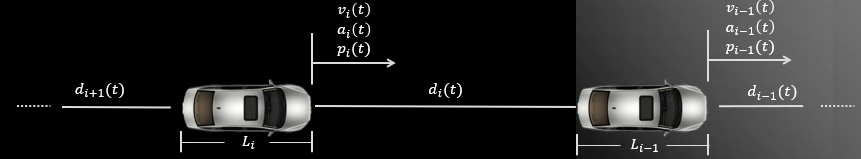
\includegraphics[width=0.8\linewidth]{assets/platoon.PNG}
    \caption{An example platoon modeled with system parameters.}
    \label{fig:platoonmodel}
\end{figure*}
\noindent As illustrated in Figure \ref{fig:platoonmodel}, for a general vehicle ($V_i$), the position of $V_i$'s front bumper is defined as $p_i$. The velocity, acceleration and control input of $V_i$ are denoted as $v_i$, $a_i$ and $u_i$.  Furthermore, the acceleration of $V_i$'s predecessor may be denoted as $a_{i-1}$. The control input for $V_i$ is defined as $u_i$ (whether $V_i$ should accelerate or decelerate).  $V_i$'s drive-train dynamics coefficient is defined as $\tau_i$, where large values of $\tau_i$ indicate larger response times for a given input $u_i$ to generate acceleration $a_i$. Lastly, the length of $V_i$ is denoted as $L_i$.  The system dynamics for $V_i$ are thus provided below as

\begin{equation}
    \begin{aligned}\label{eqn:systemparams}
        \dot{p_i(t)} &= v_i(t) \\
        \dot{v_i(t)} &= a_i(t) \\
        \dot{a_i(t)} &= -\frac{1}{\tau_i}a_i(t) + \frac{1}{\tau_i}u_i(t) \\
        \dot{a_{i-1}(t)} &= -\frac{1}{\tau_{i-1}}a_{i-1}(t) + \frac{1}{\tau_{i-1}}u_{i-1}(t)
    \end{aligned}
\end{equation}
The headway $d_i(t)$ in a CACC model is the positional difference of the current vehicle to the rear bumper of it’s leader \cite{Lin2019, leileiDRL}, which can be derived as
\begin{equation}
 \label{eqn:headway}
 d_i(t) = p_{i-1}(t) - p_i(t) - L_{i-1}.
\end{equation}
In addition, the desired headway $d_{r,i}(t)$ is defined as

\begin{equation}
    d_{r,i}(t) = r_i + h_iv_i(t), \label{eqn:deshead}
\end{equation}
where $r_i$ is the standstill distance, and $h_i$ is the time-gap for $V_i$ to maintain relative to it's predecessor $V_{i-1}$.  The position error $e_{pi}$ and the velocity error $e_{vi}$ are defined as:
\begin{equation}
\begin{aligned}
    e_{pi}(t) &= d_i(t) - d_{r,i}(t) \\
    e_{vi}(t) &= v_{i-1}(t) - v_i(t) \\
\end{aligned}
\end{equation}
Therefore, the state of $V_i$ can be defined as $x_i(t) = \begin{bmatrix}e_{pi}(t) & e_{vi}(t) & a_i(t) & a_{i-1}(t)\end{bmatrix}^\top$, and the derivative of the state is:
\begin{equation}
\begin{aligned}
    \dot{e_{pi}(t)} &= e_{vi}(t) - h_ia_i(t),\\
    \dot{e_{vi}(t)} &= a_{i-1}(t) - a_i(t), \\
    \dot{a_i(t)} &= -\frac{1}{\tau_i}a_i(t) + \frac{1}{\tau_i}u_i(t), \\
    \dot{a_{i-1}(t)} &= -\frac{1}{\tau_{i-1}}a_{i-1}(t) + \frac{1}{\tau_{i-1}}u_{i-1}(t).\\
\end{aligned}
\end{equation}
The state space formula for $V_i$ is thus given as
\begin{equation}
    \dot{x_i(t)} = A_ix_i(t) + B_iu_i(t) + C_iu_{i-1}(t), \label{eqn:stspace}
\end{equation}
where $A_i$, $B_i$, and $C_i$ are defined below as

\begin{equation} \label{eqn:systemmatrices}
    \begin{aligned}
        A_{i} &= \begin{bmatrix}
            0 & 1 & -h_i & 0 \\
            0 & 0 & -1 & 1 \\
            0 & 0 & -\frac{1}{\tau_i} & 0 \\
            0 & 0 & 0 & -\frac{1}{\tau_{i-1}}
        \end{bmatrix} \qquad
        B_{i} = \begin{bmatrix}
            0 \\ 0 \\ \dfrac{1}{\tau_i} \\ 0
        \end{bmatrix} \qquad
        C_{i} &= \begin{bmatrix}
            0 \\ 0 \\ 0 \\ \frac{1}{\tau_{i-1}}
        \end{bmatrix}.
    \end{aligned}
\end{equation}

\section{MDP Model Formulation}
The AV platooning problem can be formulated as an MDP problem, where the optimization objective is to minimize the previously defined $e_{pi}$, $e_{vi}$, $u_i$ and lastly jerk. 
\subsection{State Space}
The state space formula \eqref{eqn:stspace} can be discretized using the forward euler method giving the system equation below

\begin{equation}
    \begin{split} \label{eqn:modelBStateSpace}
        x_{i,k+1} &= A_{Di}x_{i,k} + B_{Di}u_{i,k} + C_{Di}u_{i-1, k}, \\
    \end{split}
\end{equation}





\noindent where $x_{i,k}=[e_{pi,k}, e_{vi,k}, a_{i,k}, a_{i-1,k}]$ is the observation state for the MDP problem that includes the position error $e_{pi,k}$, velocity error $e_{vi,k}$, acceleration $a_{i,k}$, and the acceleration of the predecessor vehicle $a_{i-1,k}$ at time step $k$. Moreover, $A_{Di}$, $B_{Di}$, and $C_{Di}$ are given as

\begin{equation} \label{eqn:eulerMatr}
    \begin{aligned}
        A_{Di} &= \begin{bmatrix}
            1 & T & -Th_i & 0\\
            0 & 1 & -T & T\\
            0 & 0 & -\dfrac{T}{\tau_i} + 1 & 0 \\
            0 & 0 & 0 & -\dfrac{T}{\tau_{i-1}} + 1
        \end{bmatrix} \qquad
        B_{Di} = \begin{bmatrix}
            0 \\ 0 \\ \dfrac{T}{\tau_i} \\ 0
        \end{bmatrix} \qquad
        C_{Di} &= \begin{bmatrix}
            0 \\ 0 \\ 0 \\ \frac{T}{\tau_{i-1}}
        \end{bmatrix} .
    \end{aligned}
\end{equation}

\subsection{Action Space}
Each vehicle within a single lane platoon follows the vehicle in front of it, and as such the only action the vehicle may take to maintain a desired headway is to accelerate, or decelerate. The action for the system is defined as the control input $u_{i,k}$ to the vehicle.

\subsection{Reward Function}
The design of a reward in a DDPG system is critical to provide good performance within the system.  In the considered driving scenario it is logical to minimize position error, velocity error, the amount of time spent accelerating and the jerkiness of the driving motion.  The proposed reward thus includes the normalized position error, $e_{pi,k}$, velocity error $e_{vi,k}$, control input $u_{i,k}$ and lastly the jerk. The vehicle reward $c_{i,k}$ is given below, where $a$ $b$, $c$ and $d$ are system hyperparameters.
\begin{equation} \label{eqn:rewardB}
\small
\begin{aligned}
    c_{i,k} &= -\left(a\frac{|e_{pi,k}|}{\max(e_{pi,k})} + b\frac{|e_{vi,k}|}{\max(e_{vi,k})} + c\frac{|u_{i,k}|}{\max(u_{i,k})} +  d\frac{\dot{|a_{i,k}|}}{2\max(a_{i,k})}\right) \\
    % c_{i,pl,k} &= -\frac{1}{len(V)-1}\sum_{i\epsilon V \setminus \{1\} } c_{i,k}
\end{aligned}
\end{equation}

\section{FRL DDPG Algorithm}
In this section, the design for implementing the FRL DDPG algorithm on the AV platooning problem is presented. 
\subsection{DDPG Model Description}
The DDPG algorithm is composed of an actor, $\mu$ and a critic, $Q$. The actor produces actions $a_t \in \mathbf{A}$ given some observation $x_t \in \mathbf{X}$ and the critic makes judgements on those actions while training using the Bellman equation \cite{Lillicrap2016, sutton2018reinforcement}. The actor is updated by the policy gradient \cite{Lillicrap2016}.  The critic network uses it's weights $\theta^q$ to approximate the optimal action-value function $Q(x, a|\theta^q)$ \cite{Lillicrap2016}.  The actor network uses weights $\theta^\mu$ to represent the agents current policy $\mu(x|\theta^\mu)$ for the action-value function \cite{Lillicrap2016}.  The actor $\mu(x): \mathbf{X} \xrightarrow{} \mathbf{A}$ maps the observation to the action.  Experience replay is used to mitigate the issue of training samples not being independent and identically distributed due to their generation from sequential explorations \cite{Lillicrap2016}.  Two additional models, the target actor $\mu'$ and critic $Q'$ are used in DDPG to stabilize the training of the actor and critic networks by updating parameters slowly based on the target update coefficient $\tau$.  A sufficient value of $\tau$ is chosen such that stable training of $\mu$ and $Q$ is observed.  Figure \ref{fig:ddpgdraw} provides a high level simplified overview of how the DDPG algorithm interacts with a single vehicle in a platoon.  

\begin{figure}[H]
    \centering
    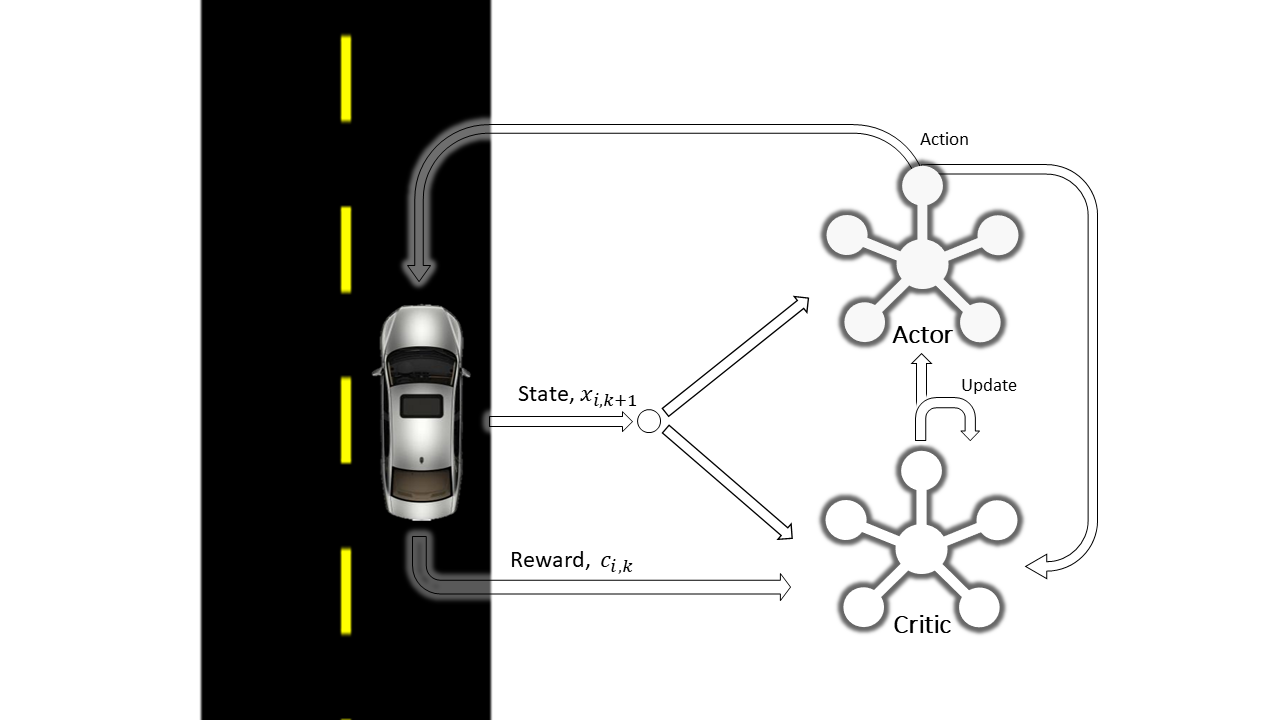
\includegraphics[width=0.6\linewidth]{assets/ddpg.PNG}
    \caption{High level flow diagram of the DDPG model for a general vehicle $V_i$ in a platoon.}
    \label{fig:ddpgdraw}
\end{figure}

\subsection{Inter and Intra FRL}
Modifications to the base DDPG algorithm are needed in order to implement Inter-FRL and Intra-FRL.  In order to implement FedAvg the following modifications are required:

\begin{enumerate}
    \item An FRL server: responsible for averaging the system parameters for use in a global update
    \item Model weight aggregation: storing of each model's weights for use in aggregation
    \item Model gradient aggregation: storing of each model's gradients for use in aggregation
\end{enumerate}

In order to perform FRL, it has been proven that including an update delay between global FRL updates is beneficial for performance \cite{Lim2020}. In addition, turning off FRL partway through training is important to allow each agent to refine their models independently of each other such that they can perform best with respect to their environments \cite{Lim2020}.  Lastly, it has also been shown that global updates and local updates should not be performed in the same episode \cite{Liang2019}.  

Two methods of aggregation are implemented in the system design, Inter-FRL (see Figure \ref{fig:interfrl}), and Intra-FRL (see Figure \ref{fig:intrafrl}).  The proposed system is capable of aggregating both the model weights and gradients for each model so that either type of parameter may be averaged for use in global updates.  The FRL server has the responsibility of averaging the parameters (model weights or gradients) across each agent in the system. 

\begin{figure}[H]
    \centering
    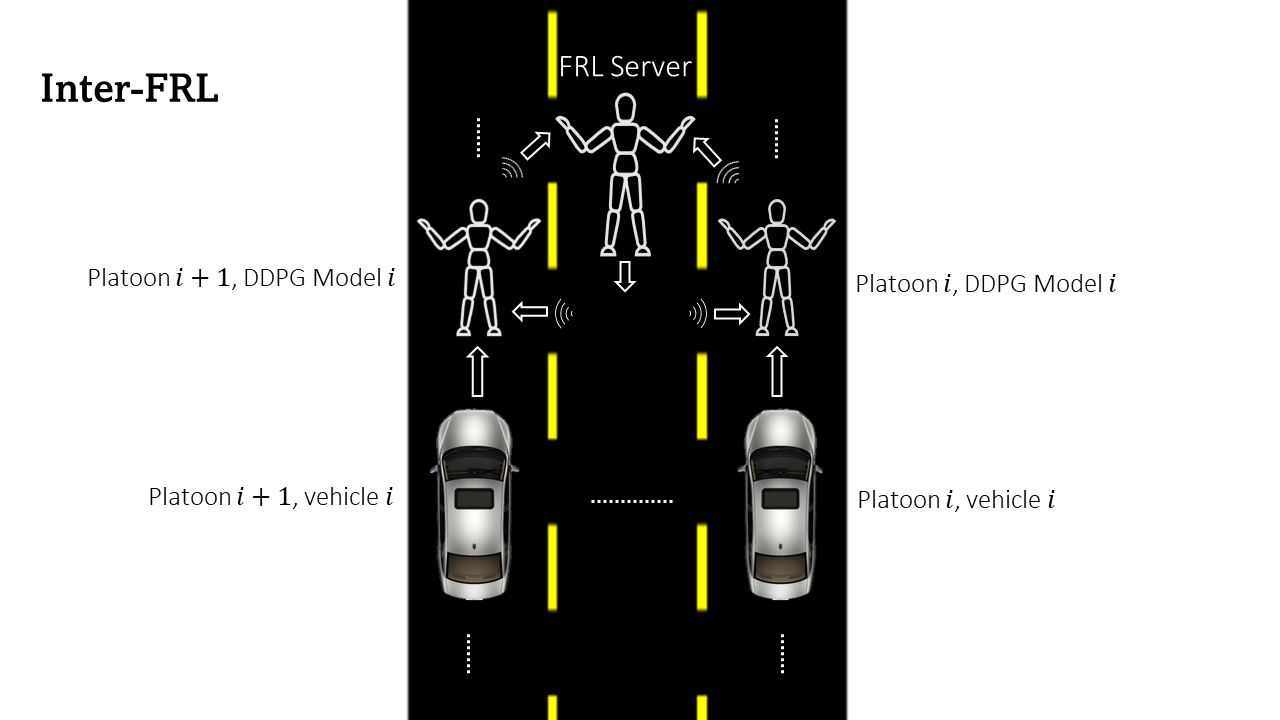
\includegraphics[width=0.69\linewidth]{assets/interfrl.PNG}
    \caption{Inter-FRL.}
    \label{fig:interfrl}
\end{figure}
\begin{figure}[H]
    \centering
    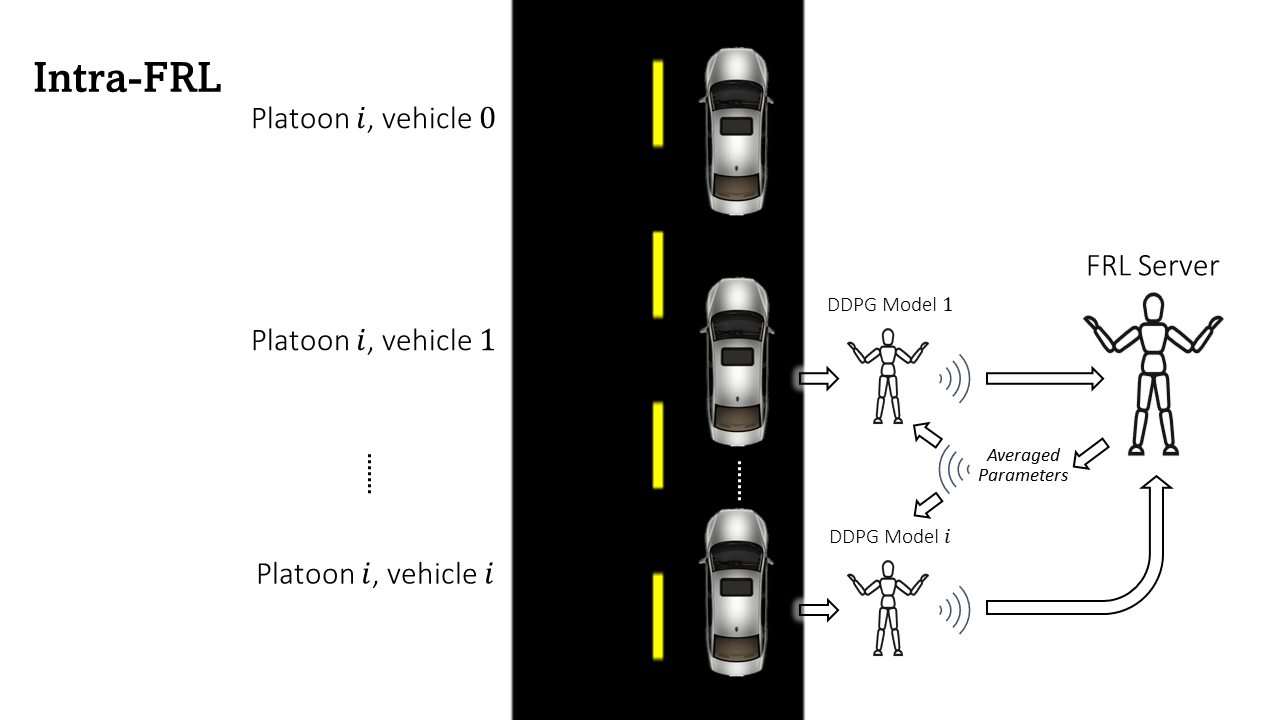
\includegraphics[width=0.69\linewidth]{assets/intrafrl.PNG}
    \caption{Intra-FRL.}
    \label{fig:intrafrl}
\end{figure}


The pseudo-code for the Inter/Intra-FRL algorithm is presented in Algorithm 1. The system is designed to allow the training of any number of equal length platoons.  At the lowest level, a DDPG agent exists for each vehicle in each platoon. As such, a DRL model must be initialized for each vehicle in the whole system.  Each DDPG agent trains separately from the others before data upload to the FRL server. Federated averaging is applied at a given time delay known as the FRL update delay, while being terminated at a given episode as defined by the cutoff ratio as seen in Table \ref{tab:frlhyps}. Currently, Algorithm 1 is synchronous, and the FRL server is also synchronous.  

\IncMargin{1em}
\begin{algorithm}
% \SetAlgoNoLine%
\footnotesize
\For{each platoon $p \in platoons$}{
    \For{$v\in vehicles$}{
        initialize replay buffer $R_{i}$\;
        initialize actor $\mu_{i}$, critic $Q_{i}$, target actor $\mu'_{i}$, target critic $Q'_{i}$\;
    }
}
\BlankLine
\For{$episode \in training\_episodes$}{
    \For{$p \in platoons$}{
        collect all vehicles states $x_{i,k}$ from $p$\;
    }
    \For{$step \in steps\_per\_episode$}{
        \For{$p\in platoons$}{
            \For{$v\in vehicles$}{
                collect actions $u_{i,k}$ from actor\;
            }
            advance the platoon $p$, with $u_{i,k}$\;
            collect $(x_{i,k}, x_{i,k+1}, c_{i,k}, terminal)$ from $p$\;
        }
        \For{$p\in platoons$}{
            \For{$v\in vehicles$}{
                add $(x_{i,k}, x_{i,k+1}, c_{i,k}, terminal)$ to replay buffer $R_{i}$\;
                \If{FRL update is not required}{
                    train $\mu_{i}$, $Q_{i}$, $\mu'_{i}$, $Q'_{i}$ locally\;
                }
                append gradients of $\mu_{i}$ and $Q_{i}$ to all\_gradients\;
                append weights of $\mu_{i}$ and $Q_{i}$ to all\_weights\;
            }
        }
        \If{FRL update required}{
            \If {gradient averaging enabled} {
                avg\_gradients $\xleftarrow{}$ global\_update(all\_gradients)\;
                train $\mu_{i}$, $Q_{i}$ using avg gradients\;
            }
            \If {weight averaging enabled} {
                avg\_weights $\xleftarrow{}$ global\_update(all\_weights)\;
                update weights $\mu_{i}$, $Q_{i}$, $\mu'_{i}$, $Q'_{i}$ using avg weights\;
            }
        }
    }
}
\BlankLine
\SetKwProg{Fn}{Function}{ is}{end}
\Fn{global\_update(params)}{
    upload params to FRL server\;
    collect averaged params from FRL server\;
    return averaged params\;
}
\caption{FRL applied to an AV platoon.}
\end{algorithm}\DecMargin{1em}


